\chapter{Perancangan Sistem}
CCGtown dibangun dengan menggunakan bahasa pemrograman Python dan JavaScript.
Adapun \textit{framework} yang digunakan adalah Django.
Versi awal CCGtown merupakan sebuah \textit{proof-of-concept} dari
\textit{open source graphical annotation tool} berbasis web yang dilengkapi dengan fitur
penganotasian semi-otomatis.
Bahasa pemrograman Python digunakan karena sebagian besar \textit{library} untuk CCG
sudah tersedia di PyPi \footnote{\url{https://pypi.org/}}.
Salah satu \textit{library} penting yang digunakan sebagai dasar dari fitur penganotasian
semi-otomatis adalah NTLK \footnote{\url{http://www.nltk.org/}}.
Selanjutnya, Django digunakan untuk mempercepat proses pengembangan aplikasi.
Adapun JavaScript digunakan untuk menjadikan CCGtown aplikasi berbasis web yang interaktif.

Alur kerja CCGtown pada umumnya adalah (1) pengguna melakukan registrasi, (2) pengguna
melakukan \textit{login} ke sistem, (3) pengguna membuat proyek baru, (4) pengguna
menambahkan kalimat yang ingin dianotasi, (5) pengguna melakukan anotasi kemudian melakukan
\textit{generate} CCG \textit{derivation} dan/atau melakukan modifikasi
\textit{derivation}-nya apabila diperlukan, dan (6) pengguna melakukan \textit{export}
setelah selesai melakukan anotasi. Alur kerja tersebut mempengaruhi desain sistem dari
CCGtown. Salah satunya adalah desain dari \textit{database} yang akan digunakan.


\section{Desain Database}
CCGtown menggunakan PostgreSQL sebagai
DBMS\footnote{Database Management System}-nya.
Hal ini karena PostgreSQL memiliki kemampuan untuk menyimpan struktur data
JSON\footnote{JavaScript Object Notation} sehingga memudahkan CCGtown untuk menyimpan
format JSON dari CCG \textit{derivation} yang telah dimanipulasi oleh pengguna melalui
fitur \textit{editable CCG derivation}.
PostgreSQL juga memiliki banyak fitur lain termasuk di antaranya dukungan
dari \textit{non-relational database model} (seperti \textit{multi-model graph})
sehingga apabila di waktu yang akan datang CCGtown memerlukan perubahan signifkan
terhadap desain \textit{database}-nya tidak perlu mengganti DBMS yang digunakan.
Fitur lain seperti \textit{function} dan \textit{procedure} juga akan sangat membantu
pengembangan CCGtown di waktu yang akan datang.

CCGtown versi awal sejatinya hanya membutuhkan tiga tabel saja yaitu tabel
\textit{accounts} untuk menyimpan pengguna yang terdaftar, tabel
\textit{projects} untuk menyimpan proyek-proyek yang sudah dibuat, dan tabel
\textit{sentences} untuk menyimpan kalimat-kalimat yang akan dianotasikan.
Tiga tabel tersebut sudah cukup untuk membangun \textit{proof-of-concept} dari
alat anotasi CCG yang akan dibangun. Adapun
ERD\footnote{Entity Relationship Diagram}-nya dapat dilihat pada Gambar\ref{erd-1}.

\begin{figure}\centering\small
  \scalebox{.75}{
  \begin{tikzpicture}[node distance=1.5cm, every edge/.style={link}]
    \node[entity] (acc) {Accounts};
    \node[attribute] (acc-id) [above=of acc] {\key{ID}} edge (acc);
    \node[attribute] (acc-uuid) [above right=of acc] {\key{UUID}} edge (acc);
    \node[attribute] (acc-email) [right=of acc] {Email} edge (acc);
    \node[attribute] (acc-password) [below right=of acc] {Password} edge (acc);

    \node[relationship] (creates) [left=of acc] {Creates} edge (acc);

    \node[entity] (prj) [below=of creates] {Projects} edge (creates);
    \node[attribute] (prj-id) [above right=of prj] {\key{ID}} edge (prj);
    \node[attribute] (prj-uuid) [above left=of prj] {\key{UUID}} edge (prj);
    \node[attribute] (prj-author) [left=of prj] {Author ID} edge (prj);
    \node[attribute] (prj-name) [below left=of prj] {Name} edge (prj);
    \node[attribute] (prj-status) [below=of prj] {Status} edge (prj);
    \node[attribute] (prj-rules) [below right=of prj] {Rules} edge (prj);

    \node[relationship] (adds) [right=0.5cm and 2cm of prj] {Adds} edge (prj);

    \node[entity] (snt) [below=of adds] {Sentences} edge (adds);
    \node[attribute] (snt-id) [left=of snt] {\key{ID}} edge (snt);
    \node[attribute] (snt-uuid) [below left=of snt] {\key{UUID}} edge (snt);
    \node[attribute] (snt-project) [below=of snt] {Project ID} edge (snt);
    \node[attribute] (snt-words) [below right=of snt] {Words} edge (snt);
    \node[attribute] (snt-cats) [right=of snt] {Categories} edge (snt);
    \node[attribute] (snt-deriv) [above right=of snt] {Derivations} edge (snt);
  \end{tikzpicture}
  }
  \caption{Conceptual Entity Relationship Diagram (ERD) CCGtown}
  \label{erd-1}
\end{figure}

Masing-masing tabel memiliki dua \textit{key} yaitu $ID$ dan
$UUID$\footnote{Universally Unique IDentifier}.
$ID$ merupakan \textit{primary key} \textit{integer} dengan \textit{auto increment}
yang berfungsi sebagai \textit{identifier} untuk melakukan operasi
\textit{update} maupun \textit{delete}.
Adapun $UUID$ merupakan \textit{indexed column} yang berfungsi sebagai
\textit{indentifier} publik (dapat dilihat oleh pengguna melalui URL)
yang mana digunakan untuk operasi \textit{read}.
$ID$ tidak digunakan sebagai \textit{identifier} publik karena pengguna dapat
melakukan \textit{brute-force} untuk mencari proyek ataupun kalimat berdasarkan
$ID$ yang bukan miliknya.
Demikian itu alasan ditambahkannya atribut $UUID$.
Alasan kenapa CCGtown tetap menyimpan kolom $ID$ adalah karena $ID$ nantinya akan
digunakan untuk membuat \textit{pagination}.

Pada tabel $accounts$, selain $ID$ dan $UUID$ juga memiliki atribut $email$ dan
$password$. Masing-masing atribut tersebut menggunakan tipe data \textit{string}
atau VARCHAR di PostgreSQL.
Tabel $accounts$ memiliki hubungan \textit{one-to-many} terhadap tabel $projects$.
Adapun atribut tabel $projects$ adalah $author\_id$, $name$, $status$, dan $rules$.
Atribut $author\_id$ merupakan \textit{foreign key} (\textit{indexed}) yang
mengarah kepada tabel $accounts$ dan tipe data yang digunakan sama dengan
atribut $ID$ yang terdapat di tabel $accounts$.
Atribut $name$ menggunakan tipe data \textit{string} (VARCHAR).
Atribut $status$ menggunakan tipe data \textit{integer} yang berperan sebagai
\textit{enum} ($0$ = \textit{just created}, $1$ = \textit{in progress},
$2$ = \textit{finished}, dan $3$ = \textit{dropped}).
Tabel $projects$ memiliki hubungan \textit{one-to-many} terhadap tabel $sentences$.
Adapun atribut tabel $sentences$ adalah $project\_id$, $words$, $categories$, dan
$derivations$. Atribut $project\_id$ merupakan \textit{foreign key}
(\textit{indexed}) yang mengarah kepada tabel $projects$ dan tipe data yang digunakan
sama dengan atribut $ID$ yang terdapat di tabel $projects$.
Sisanya, atribut $words$, $categories$, dan $derivations$ menggunakan tipe data JSON.


\section{Desain Sistem}
CCGtown sejatinya memiliki desain sistem yang cukup sederhana.
Fungsionalitas yang akan didukung untuk versi awal adalah (1) \textit{register} dan
\textit{login}, (2) manajemen proyek (CRUD\footnote{Create, Read, Update, Delete}
), (3) dan manajemen kalimat (CRUD).
Pada manajemen kalimat, CCGtown menggunakan JavaScript untuk membuat pembuatan
maupun perubahan CCG \textit{derivation} menjadi lebih interaktif.
Selain tiga fungsionalitas tersebut, CCGtown juga menambahkan fungsionalitas tambahan
seperti \textit{auto-assign category} yang dilakukan di sisi \textit{frontend}.
Kemudian, CCGtown juga menambahkan fungsionalitas tambahan di sisi \textit{backend}
yaitu CCG \textit{derivation generator} dengan memanfaatkan \textit{library} NLTK
dan kemampuan untuk melakukan \textit{export} CCG \textit{derivation} yang disimpan
di \textit{database}.

Pengguna harus terdaftar terlebih dahulu sebelum dapat melaukan anotasi sehingga
langkah awal yang harus dibangun adalah fungsionalitas \textit{register}.
Alur proses pendaftaran pengguna dapat dilihat pada Gambar \ref{flowchart:register}.
Berhubung fokus saat ini adalah \textit{proof-of-concept}, informasi yang dibutuhkan
untuk mendaftar hanyalah \textit{email} dan \textit{password}. Adapun
\textit{password confirmation} digunakan untuk memvalidasi \textit{password}
sehingga dapat mengurangi risiko pengguna melupakan
\textit{password}-nya yang baru saja di-\textit{input}.
Saat pengguna melakukan pendaftaran, sistem akan memeriksa apakah \textit{email} yang
didaftar sudah terdapat di \textit{database}.
Apabila sudah terdaftar, pengguna akan dialihkan ke halaman \textit{register} kembali
dan mendapatkan \textit{flash message} dengan keterangan "email sudah terdaftar".
Sebaliknya, sistem akan melakukan \textit{input} data tersebut ke dalam \textit{database}
lalu mengalihkan pengguna ke halaman \textit{login}.
Ketika dialihkan ke halaman \textit{login}, pengguna akan melihat \textit{flash message}
dengan keterangan "pengguna berhasil didaftarkan".
Pada tahap ini pengguna sudah dapat melakukan \textit{login} ke dalam sistem CCGtown.

\begin{figure}\centering\small
  \scalebox{.75}{
	\begin{tikzpicture}[node distance=2cm]
    \node (start) [cloud] {Start};
    \node (input) [io, below of=start, yshift=0.5cm] {\textit{Input email, password,} dan \textit{password confirmation}};
    \node (check) [process, below of=input, yshift=0.5cm] {Mencari pengguna berdasarkan \textit{email}};
    \node (is-registered) [decision, below of=check, yshift=-1.25cm] {\textit{Email} sudah terdaftar?};
    \node (registered) [process, right of=is-registered, yshift=0cm, xshift=4.5cm] {\textit{Redirect} ke halaman \textit{register}};
    \node (registering) [process, below of=is-registered, yshift=-1.75cm] {\textit{Input} informasi pengguna ke \textit{database}};
    \node (redirect) [process, below of=registering, yshift=0.5cm] {\textit{Redirect} ke halaman \textit{login}};
    \node (stop) [cloud, below of=redirect, yshift=0.5cm] {Stop};

    \draw [arrow] (start) -- (input);
    \draw [arrow] (input) -- (check);
    \draw [arrow] (check) -- (is-registered);
    \draw [arrow] (is-registered) -- node[anchor=south]{Ya} (registered);
    \draw [arrow] (registered) -- +(3,0) |- (input);
    \draw [arrow] (is-registered) -- node[anchor=east]{Tidak} (registering);
    \draw [arrow] (registering) -- (redirect);
    \draw [arrow] (redirect) -- (stop);
  \end{tikzpicture}
  }
	\caption{Alur proses pendaftaran pengguna.}
  \label{flowchart:register}
\end{figure}

Pada proses "\textit{input} informasi pengguna ke \textit{database}" CCGtown melakukan
\textit{password hashing} dengan menggunakan Bcrypt.
Informasi sensitif seperti \textit{password} sebaiknya tidak disimpan sebagai
\textit{plain text}. Demikian itu CCGtown menggunakan \textit{password hashing}.
Apabila hal buruk terjadi seperti misalnya \textit{data breach} (kebocoran data),
\textit{password} pengguna tidak dapat langsung digunakan.
Peretas perlu mencari cara untuk memecahkan \textit{password} tersebut.
Bcrypt merupakan skema \textit{password hashing} berbasis Blowfish \textit{block cipher}
yang didesain untuk lebih \textit{resistant} terhadap serangan \textit{brute-force}
\cite{bcrypt}.
Serangan \textit{brute-force} merupakan upaya peretas untuk menebak \textit{password}
dengan cara membuat \textit{wordlist} yang kemudian dicocokkan dengan \textit{hash}
yang terbentuk satu-demi-satu.
Meskipun terjadi \textit{data breach}, peretas perlu usaha ekstra untuk dapat menebak
\textit{password} dari satu pengguna.
Hal ini mengurangi kerugian yang akan dialami oleh CCGtown apabila \textit{data breach}
benar-benar terjadi.

Selanjutnya, setelah melakukan registrasi, pengguna dapat melakukan \textit{login} ke
sistem CCGtown.
Proses yang dilakukan pada umumnya sama dengan aplikasi web yang memiliki
kemampuan \textit{register} dan \textit{login}. Alur proses \textit{login} dapat dilihat
pada Gambar \ref{flowchart:login}.
Setelah pengguna melakukan \textit{input} \textit{email} dan \textit{password}-nya,
CCGtown akan melakukan pencarian di \textit{database} apakah \textit{email} yang
diberikan terdaftar. Apabila tidak terdaftar, pengguna akan dialihkan ke halaman
\textit{login} dan diberikan \textit{flash message} "\textit{Email} dan/atau
\textit{password} tidak cocok". Pesan ini diberikan agar peretas tidak dapat mencari
tahu \textit{email} mana saja yang sudah terdaftar. Selanjutnya, apabila akun
dengan \textit{email} tersebut ada, maka langkah selanjutnya adalah mencocokkan
\textit{password} yang diberikan oleh pengguna dan \textit{password} yang telah
disimpan di \textit{database}. Kemudian, sistem melakukan Bcrypt \textit{sync}.
Apabila tidak berhasil, pengguna akan dialihkan ke halaman \textit{login}
dan diberikan \textit{flash message} "\textit{Email} dan/atau \textit{password}
tidak cocok". Sebaliknya, pengguna akan dialihkan ke halaman Projects yang berisi
daftar proyek yang telah dibuat sebelumnya.

\begin{figure}\centering\small
  \scalebox{.75}{
	\begin{tikzpicture}[node distance=2cm]
    \node (start) [cloud] {Start};
    \node (input) [io, below of=start, yshift=0.5cm] {\textit{Input email} dan \textit{password}};
    \node (check) [process, below of=input, yshift=0.5cm] {Mencari pengguna berdasarkan \textit{email}};
    \node (is-registered) [decision, below of=check, yshift=-1.25cm] {\textit{Email} sudah terdaftar?};
    \node (not-registered) [process, left of=is-registered, yshift=0cm, xshift=-4.5cm] {\textit{Redirect} ke halaman \textit{login}};
    \node (logging-in) [process, below of=is-registered, yshift=-1.75cm] {Mencocokkan \textit{password} dengan Bcrypt \textit{sync}};
    \node (is-matched) [decision, below of=logging-in, yshift=-1.25cm] {\textit{Password} cocok?};
    \node (redirect) [process, below of=is-matched, yshift=-1.75cm] {\textit{Redirect} ke halaman Projects};
    \node (stop) [cloud, below of=redirect, yshift=0.5cm] {Stop};

    \draw [arrow] (start) -- (input);
    \draw [arrow] (input) -- (check);
    \draw [arrow] (check) -- (is-registered);
    \draw [arrow] (is-registered) -- node[anchor=south]{Tidak} (not-registered);
    \draw [arrow] (not-registered.north) -- +(0,0) |- (input);
    \draw [arrow] (is-registered) -- node[anchor=east]{Ya} (logging-in);
    \draw [arrow] (logging-in) -- (is-matched);
    \draw [arrow] (is-matched.west) -| +(-4.6,0) -- node[anchor=east]{Tidak} (not-registered.south);
    \draw [arrow] (is-matched) -- node[anchor=east]{Ya} (redirect);
    \draw [arrow] (redirect) -- (stop);
  \end{tikzpicture}
  }
	\caption{Alur proses \textit{login} ke sistem CCG.}
  \label{flowchart:login}
\end{figure}

Pada halaman Projects, pengguna dapat membuat proyek atau menghapus proyek.
Tidak ada fungsionalitas spesial di halaman Projects selain CRUD pada umumnya.
Satu pengguna dapat membuat banyak proyek. Tidak ada larangan tertentu terhadap penamaan
proyek. Namun, sangat disarankan memberikan nama proyek yang deskriptif seperti misalnya
"\textit{Wide-range Indonesian Dataset}". Setiap proyek memiliki status yang berbeda-beda.
Proyek yang baru saja dibuat akan memiliki status \textit{just created}.
Hal ini untuk memudahkan \textit{annotator} mencari proyek mana yang baru akan dikerjakan,
proyek mana yang sedang dikerjakan, proyek mana yang sudah selesai dikerjakan, atau
proyek mana yang tidak jadi dikerjakan. Proyek yang telah dibuat dapat disunting maupun
dihapus. Proyek yang dihapus tidak dapat dikembalikan (\textit{undo}).
Adapun penyuntingan proyek terjadi di halaman Editor.

Pada halaman Editor, pengguna dapat menyunting informasi proyek seperti nama proyek,
status proyek, dan \textit{rules} yang akan digunakan untuk melakukan \textit{generate}
CCG \textit{derivation} via NTLK. Selain itu, pengguna juga dapat menambahkan kalimat
baru yang akan dianotasi. Pengguna dapat menambahkan lebih dari satu kalimat sekaligus.
Kalimat-kalimat tersebut akan di-\textit{tokenize} menggunakan \textit{library} NLTK.
Ekstensi yang digunakan untuk proses \textit{tokenize} ini adalah punkt.
Setelah itu, barulah pengguna dapat melakukan penganotasian terhadap kalimat-kalimat yang
telah ditambahkan. Terdapat dua cara untuk memberikan anotasi yaitu secara langsung di
halaman Editor atau dapat juga dilakukan di Editable CCG Modal.
Saat ini CCGtown belum mendukung penganotasian terhadap \textit{compound words}.
CCGtown saat ini juga belum mendukung penganotasian CCG dengan semantik.
Versi awal CCGtown hanya mendukung penganotasian CCG secara sintaksis saja.

Setelah semua kata dalam suatu kalimat diberikan anotasi, pengguna dapat melakukan
\textit{generate} CCG \textit{derivation}. Hal ini dapat dilakukan berkat bantuan
\textit{library} NLTK. Kami mengambil sebuah $rules$ dari tabel $projects$ dan kemudian
kami mengambil semua $words$ serta $categories$ dari tabel $sentences$ yang merupakan
bagian dari proyek tersebut. Kolom $words$ merupakan kumpulan kata dari kalimat yang telah
di-\textit{tokenize}. Adapun kolom $categories$ merupakan anotasi CCG \textit{category}-nya.
\textit{Pseudocode} untuk \textit{generate} CCG \textit{derivation} dapat dilihat pada
Kode \ref{code:ccg-gen} dengan asumsi anotasi yang diberikan absah (dapat dibuat CCG
\textit{derivation}-nya). Kode $next$ tersebut akan mengambil satu dari banyak
kemungkinan \textit{derivation} yang dapat dibuat. Contoh \textit{object} yang
di-\textit{return} dapat dilihat pada Kode \ref{code:ccg-gen-example}.
Untuk kepentingan \textit{rendering} di sisi \textit{frontend}, \textit{key} seperti
$from$ dan $to$ sangat diperlukan. \textit{Key} $from$ dan \textit{key} $to$
merepresentasikan \textit{index} posisi terhadap \textit{array} $words$.
Dengan bantuan kedua \textit{key} tersebut, \textit{frontend} dapat melakukan kalkulasi
posisi masing-masing elemen yang terdapat di \textit{object} $derivations$.

\begin{lstlisting}[
  language=python,
  firstnumber=1,
  caption={Pseudocode untuk melakukan \textit{generate} CCG \textit{derivation}.},
  label={code:ccg-gen}
]
from nltk.ccg import chart, lexicon

def generateCCGDerivation(rules, words, categories, target_words):
    lex = rules + '\n\n'
    for i in range(len(words)):
        lex += words[i] + ' => ' + categories[i] + '\n'

    lex = lexicon.parseLexicon(lex)
    parser = chart.CCGChartParser(lex, chart.DefaultRuleSet)
    result = next(parser.parse(target_words))
    derivations = makeCCGDeriv(result)

    return derivations
\end{lstlisting}

Kode \ref{code:ccg-gen-example} didapatkan dari fungsi $makeCCGDeriv$ yang terdapat pada
Kode \ref{code:ccg-gen}. Fungsi $makeCCGDeriv$ sederhananya mengambil $Tree$ yang didapatkan
dari $parser.parse$ kemudian melakukan \textit{tree traversal}. Semua \textit{leaf}, diambil
dari paling "kiri", diletakkan di elemen pertama $derivations$. Selanjutnya, kita berjalan
melalui \textit{parent} dari \textit{leaf} tersebut hingga ke \textit{root} mencari bentuk CCG
\textit{derivation}-nya. Banyaknya baris yang dibutuhkan oleh CCG \textit{derivation} dapat
dilihat dari \textit{height} yang dimiliki oleh $Tree$ tersebut. Kemudian, hasil dari CCG
\textit{derivation} (umumnya berupa $S$) merupakan elemen terakhir $derivations$.
Adapun hasil \textit{render} di sisi \textit{frontend}-nya dapat dilihat pada Gambar
\ref{ui:deriv-generated}.

\begin{lstlisting}[
  language=json,
  firstnumber=1,
  caption={Contoh \textit{derivations object} yang di-\textit{return}.},
  label={code:ccg-gen-example}
]
[
  [
    { "to": 0, "from": 0, "word": "You" },
    { "to": 1, "from": 1, "word": "prefer" },
    { "to": 2, "from": 2, "word": "that" },
    { "to": 3, "from": 3, "word": "cake" }
  ],
  [
    { "to": 0, "from": 0, "category": "NP" },
    { "to": 1, "from": 1, "category": "((S\NP)/NP)" },
    { "to": 2, "from": 2, "category": "(NP/N)" },
    { "to": 3, "from": 3, "category": "N" }
  ],
  [
    { "to": 3, "from": 2, "category": "NP", "operator": ">" }
  ],
  [
    { "to": 3, "from": 1, "category": "(S\NP)", "operator": ">" }
  ],
  [
    { "to": 3, "from": 0, "category": "S", "operator": "<" }
  ]
]
\end{lstlisting}

Selain memiliki kemampuan untuk melakukan \textit{generate} CCG \textit{derivation},
CCGtown juga memiliki kemampuan untuk melakukan \textit{auto-assign} CCG \textit{category}.
Token kata yang sudah dianotasi oleh pengguna akan disimpan ke dalam suatu \textit{dictionary}.
Untuk setiap kata yang belum dianotasi, CCGtown akan memeriksa apakah token kata tersebut
sebelumnya sudah dianotasi. Apabila sudah, CCGtown akan memberikan anotasi secara otomatis.
Suatu token kata mungkin memiliki lebih dari satu anotasi. CCGtown hanya akan mengambil satu
anotasi saja. Akibatnya, pengguna sebaiknya tetap melakukan peninjauan.
Kendati demikian, setidaknya kegiatan anotasi yang repetitif dapat berkurang sehingga memudahkan
dan mempercepat proses anotasi.


\section{Pertimbangan UI/UX}
Secara keseluruhan, CCGtown memiliki halaman rumah (\textit{homepage}), halaman \textit{register},
halaman \textit{login}, halaman Projects, dan halaman Editor.
Halaman \textit{register} dan halaman \textit{login} pada dasarnya sama.
Perbedaannya hanya terdapat di jumlah \textit{field} yang diminta serta \textit{copy writting}
yang sedikit berbeda. Desain UI\footnote{User Interface} serta UX\footnote{User Experience}
CCGtown dibuat dengan fokus untuk mempermudah penggunaan \textit{annotation tool} ini.
CCGtown tidak menggunakan banyak warna. Hal ini untuk mengurangi kelelahan pada mata pengguna.
CCGtown menggunakan bahasa Inggris di antarmukanya karena target pengguna CCGtown adalah
pengguna baik dari Indonesia yang mengerti bahasa Inggris maupun pengguna dari manca negara.

CCGtown menggunakan UIKit\footnote{\url{https://getuikit.com/}} sebagai \textit{framework}
untuk melakukan implementasi desain web-nya. UIKit dipilih karena komponen-komponen yang
dibutuhkan CCGtown sudah tersedia sehingga CCGtown hanya perlu melakukan sedikit penyesuaian
seperti penambahan warna, pengaturan jarak (\textit{margin} dan \textit{padding}), dan sejenisnya.
UIKit juga sudah menyediakan kumpulan \textit{icons} yang dapat langsung digunakan.
Hal ini mengakibatkan proses pengembangan desain web CCGtown dapat diselesaikan dalam waktu yang
relatif cukup singkat.

Warna utama (\textit{primary color}) CCGtown adalah warna ungu.
Berdasarkan psikologi warna, warna ungu adalah warna fantasi dan magis.
CCGtown dapat men-\textit{generate} CCG \textit{derivation} dan melakukan \textit{auto-assign}
CCG \textit{category} sehingga memiliki sifat yang seakan-akan mengandung magi (sihir).
Selain itu, ungu menumbuhkan kreativitas dengan membangkitkan indra kita sambil mempromosikan
ketenangan yang diperlukan untuk melakukan pengamatan yang intuitif dan berwawasan.
Warna ungu banyak digunakan oleh \textit{homepage} seperti yang terlihat pada Gambar
\ref{ui:homepage}. Halaman rumah CCGtown didesain sederhana dan langsung kepada intinya.
Halaman rumah CCGtown menampilkan beberapa fitur yang dapat menjadi alasan bagi pengguna
untuk menggunakan CCGtown. Selain itu, halaman rumah CCGtown juga menampilkan demonstrasi
singkat dengan gambar animasi proses penganotasian di CCGtown. Demonstrasi singkat
diberikan untuk memberikan gambaran kepada calon pengguna tentang betapa mudahnya
menggunakan CCGtown untuk menganotasi CCG.

\begin{figure}\centering
  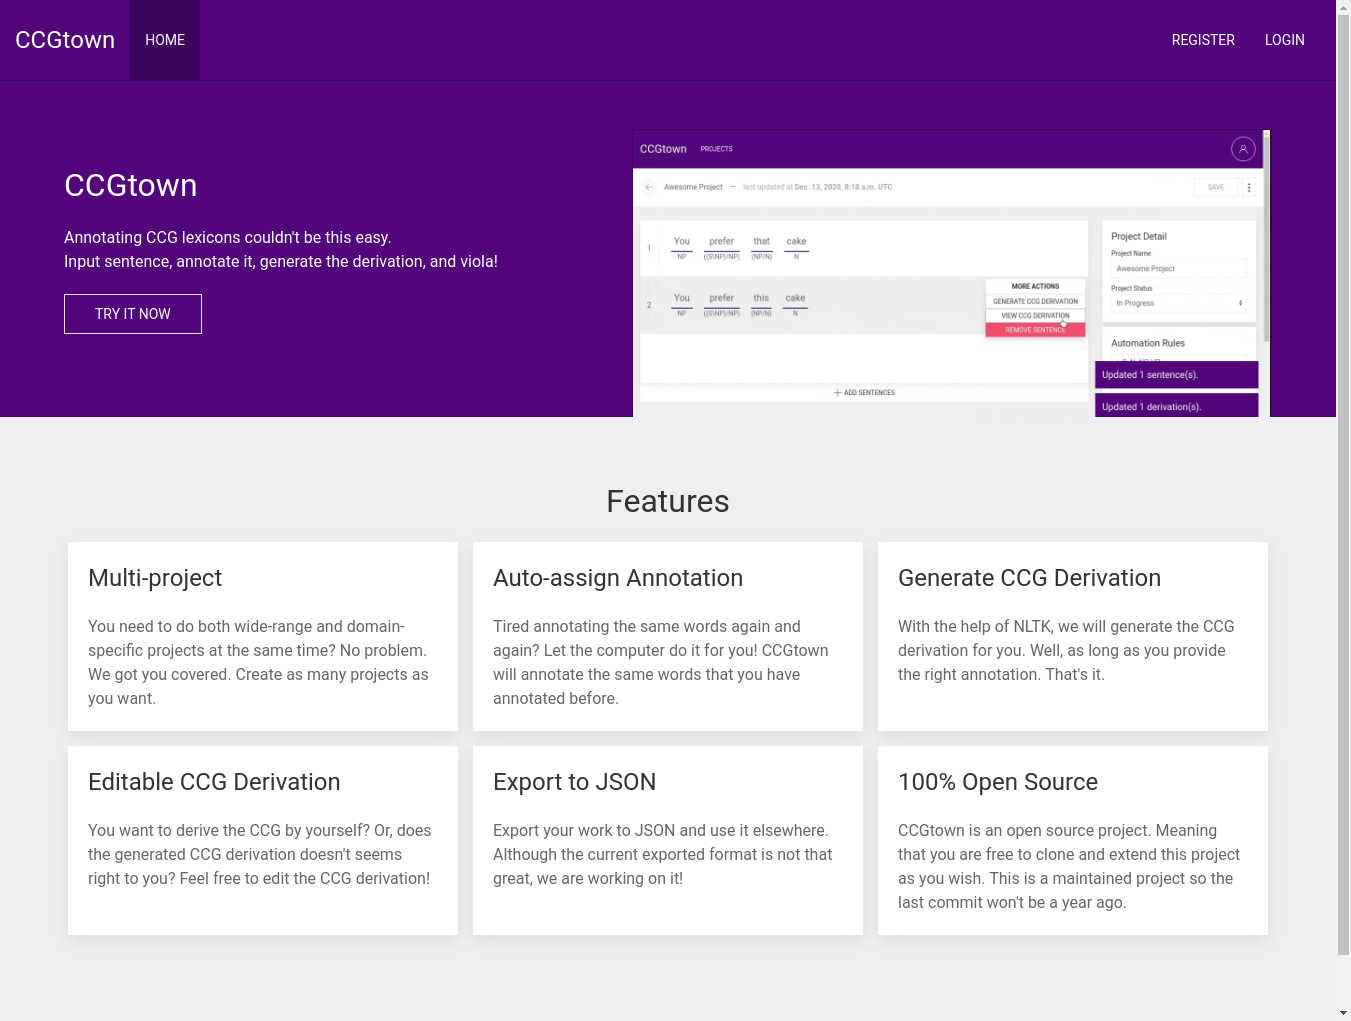
\includegraphics[width=\textwidth]{homepage}
  \caption{Antarmuka \textit{homepage} CCGtown.}
  \label{ui:homepage}
\end{figure}

\begin{figure}\centering
  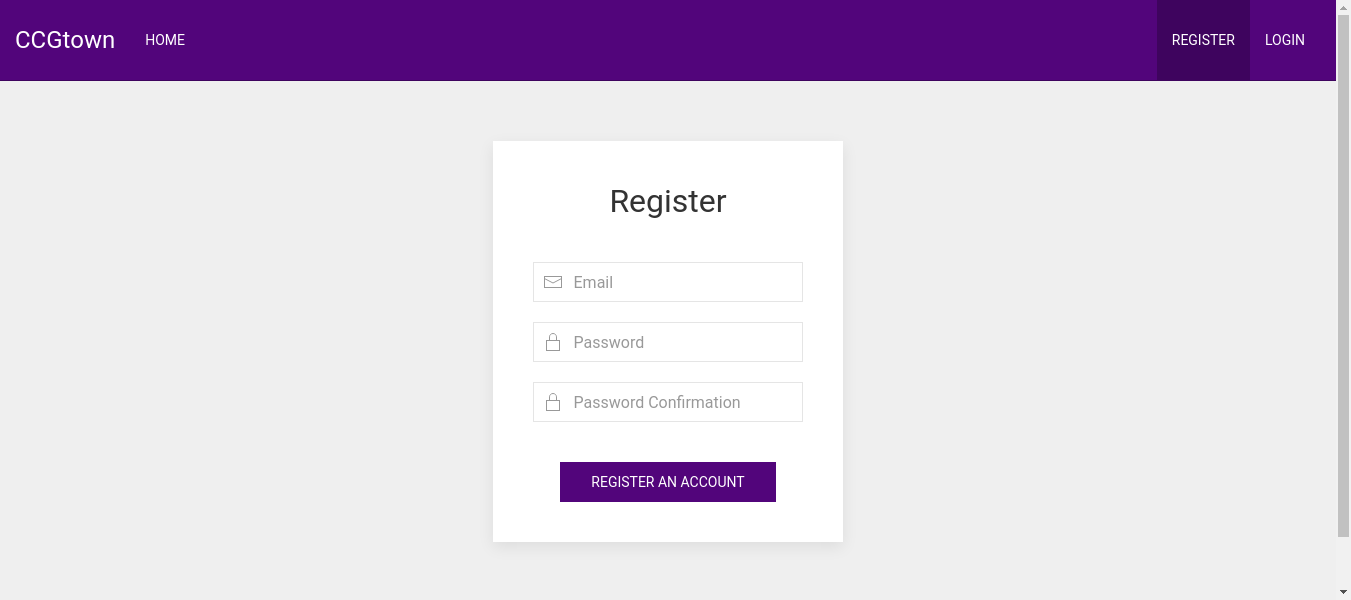
\includegraphics[width=\textwidth]{register}
  \caption{Antarmuka halaman \textit{register} CCGtown.}
  \label{ui:register}
\end{figure}

\begin{figure}\centering
  
\includegraphics[width=\textwidth]{login}
  \caption{Antarmuka halaman \textit{login} CCGtown.}
  \label{ui:login}
\end{figure}

Pada Gambar \ref{ui:register} dan Gambar \ref{ui:login}, terlihat bahwasannya halaman
\textit{register} dan halaman \textit{login} pada dasarnya sama. Pada halaman
\textit{register}, informasi yang dibutuhkan hanyalah \textit{email address} dan
\textit{password} (dengan tambahan \textit{password confirmation} untuk validasi).
Hal ini agar pengguna dapat dengan mudah mendaftar tanpa perlu mengisi banyak \textit{field}
terlebih dahulu sebelum dapat menggunakan CCGtown. Selain itu, informasi lain dari
pengguna saat ini belum dibutuhkan. Apabila terjadi perubahan mengenai data pengguna,
pengguna dapat memperbarui datanya di kemudian hari melaui halaman lain seperti halaman profil
yang mungkin saja akan ditambahkan di CCGtown versi berikutnya.

CCGtown menggunakan \textit{flash message} berupa \textit{toast} untuk setiap pesan
\textit{feedback} yang diberikan oleh sisi \textit{backend}. Sebagai contoh, pada Gambar
\ref{ui:flash-message} di bagian pojok kanan bawah merupakan pesan \textit{feedback}
yang memberikan informasi bahwasannya kombinasi \textit{email} dan/atau \textit{password}
tidak cocok sehingga pengguna tidak dapat \textit{login}. Notifikasi \textit{toast} tersebut
dapat langsung ditutup oleh pengguna atau akan hilang dengan sendirinya dalam waktu sekitar
lima detik. Penggunaan \textit{toast} yang muncul dari bawah dengan warna ungu tersebut
dapat mengalihkan perhatian pengguna sehingga pengguna menyadari pesan yang disampaikan oleh
\textit{backend} CCGtown.

\begin{figure}\centering
  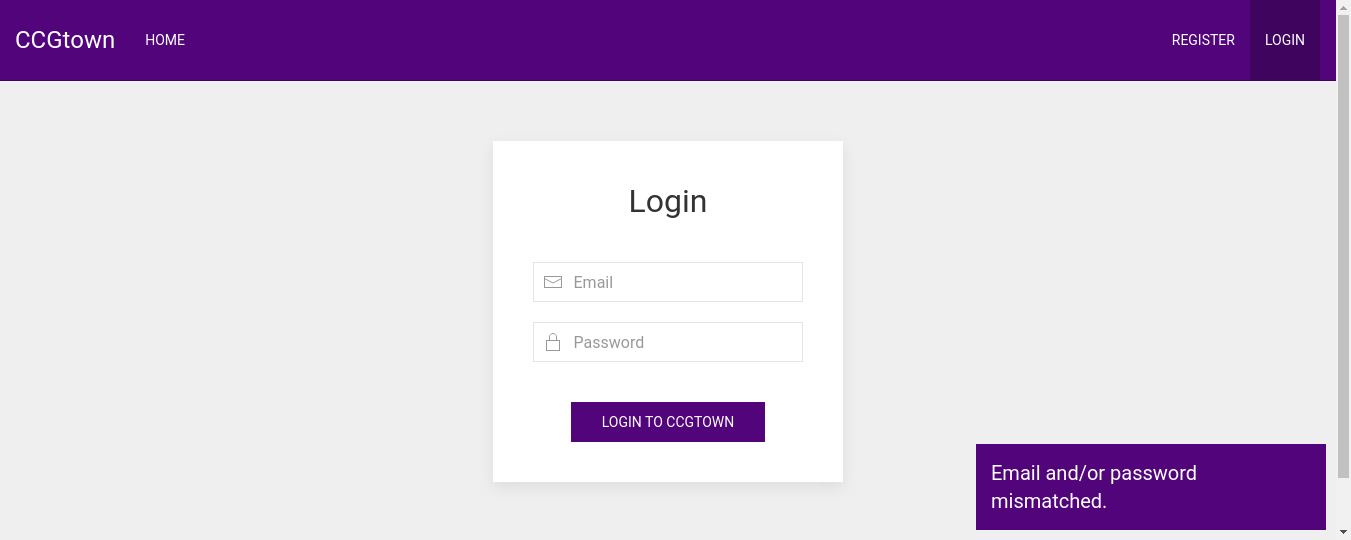
\includegraphics[width=\textwidth]{flash-message}
  \caption{Antarmuka halaman \textit{login} CCGtown dengan \textit{toast}.}
  \label{ui:flash-message}
\end{figure}

\begin{figure}\centering
  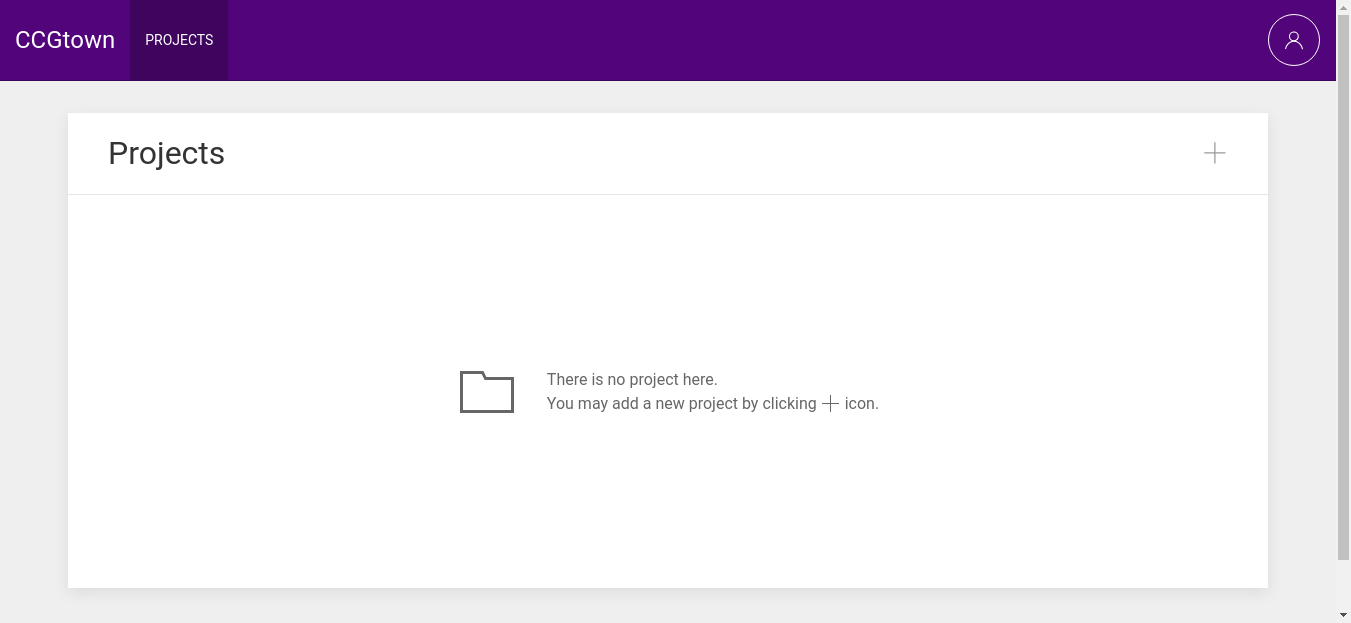
\includegraphics[width=\textwidth]{projects-empty}
  \caption{Antarmuka halaman Projects saat dalam \textit{empty state}.}
  \label{ui:projects-empty}
\end{figure}

\begin{figure}\centering
  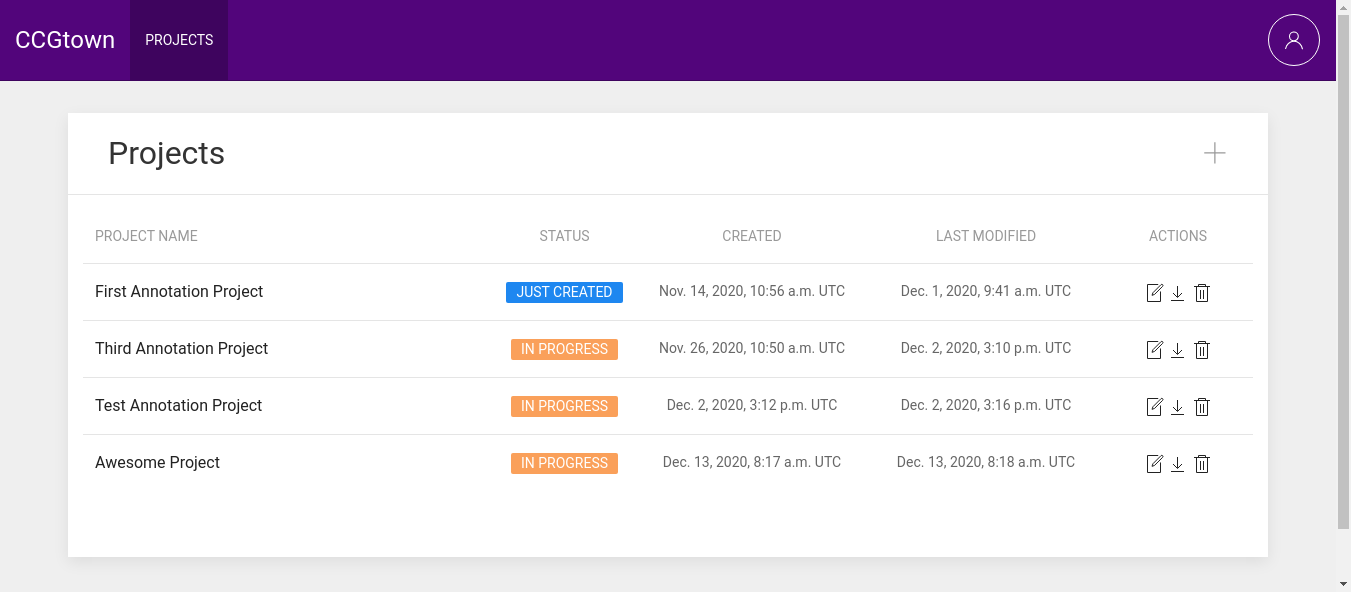
\includegraphics[width=\textwidth]{projects}
  \caption{Antarmuka halaman Projects CCGtown.}
  \label{ui:projects}
\end{figure}

\begin{figure}\centering
  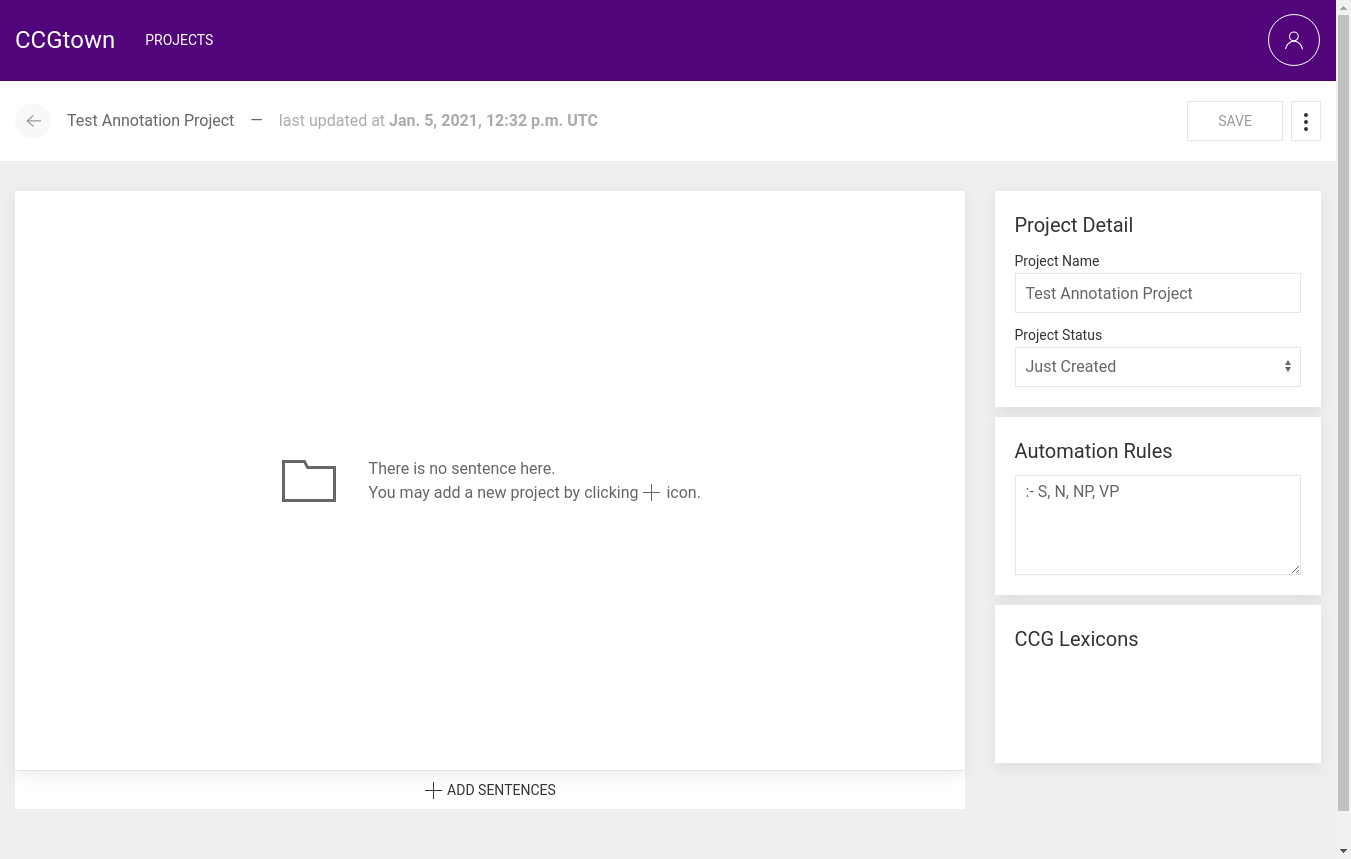
\includegraphics[width=\textwidth]{editor-empty}
  \caption{Antarmuka halaman Editor saat dalam \textit{empty state}.}
  \label{ui:editor-empty}
\end{figure}

\begin{figure}\centering
  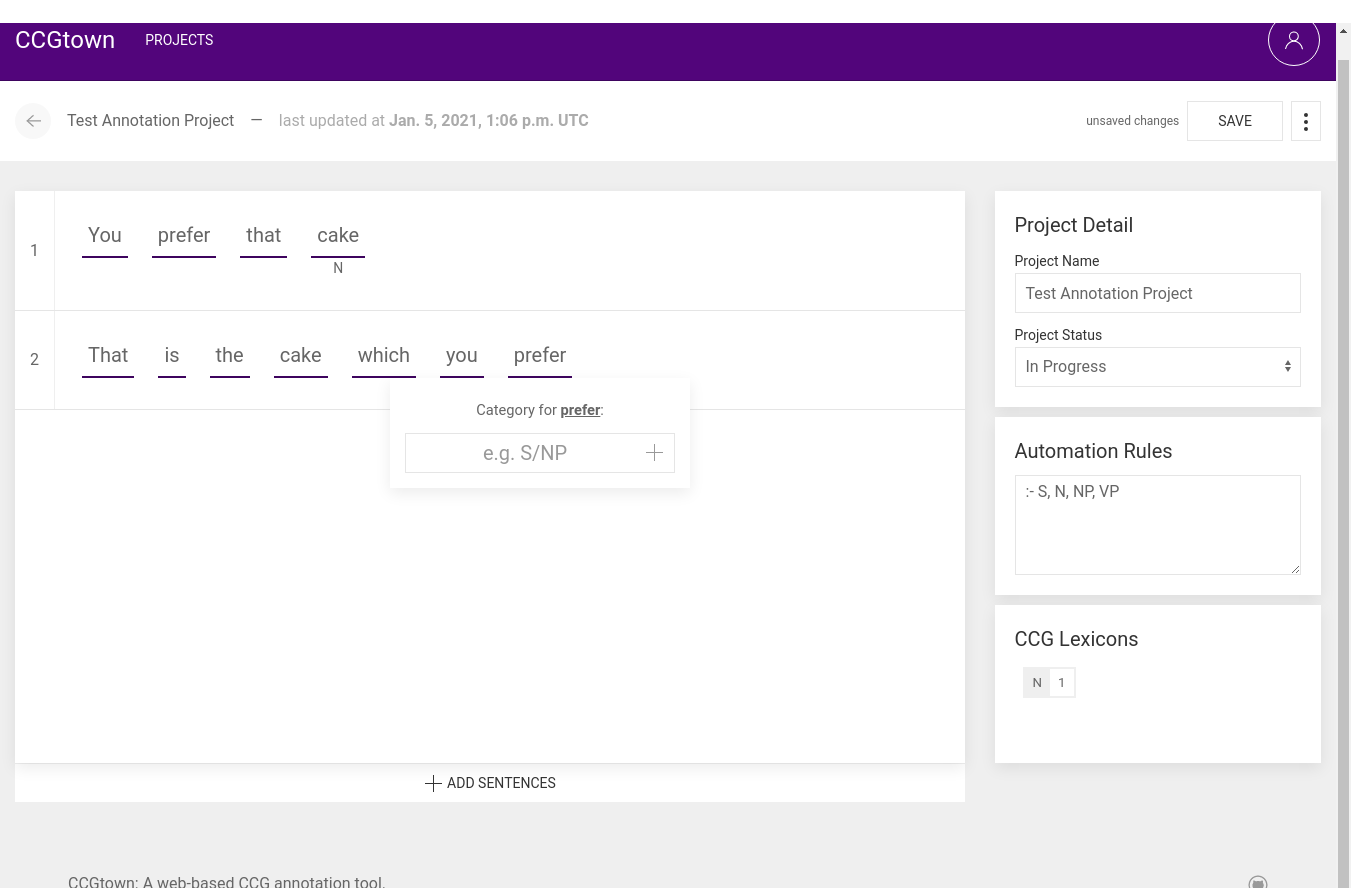
\includegraphics[width=\textwidth]{editor-annotating}
  \caption{Antarmuka halaman Editor saat melakukan penganotasian.}
  \label{ui:editor-annotating}
\end{figure}

\begin{figure}\centering
  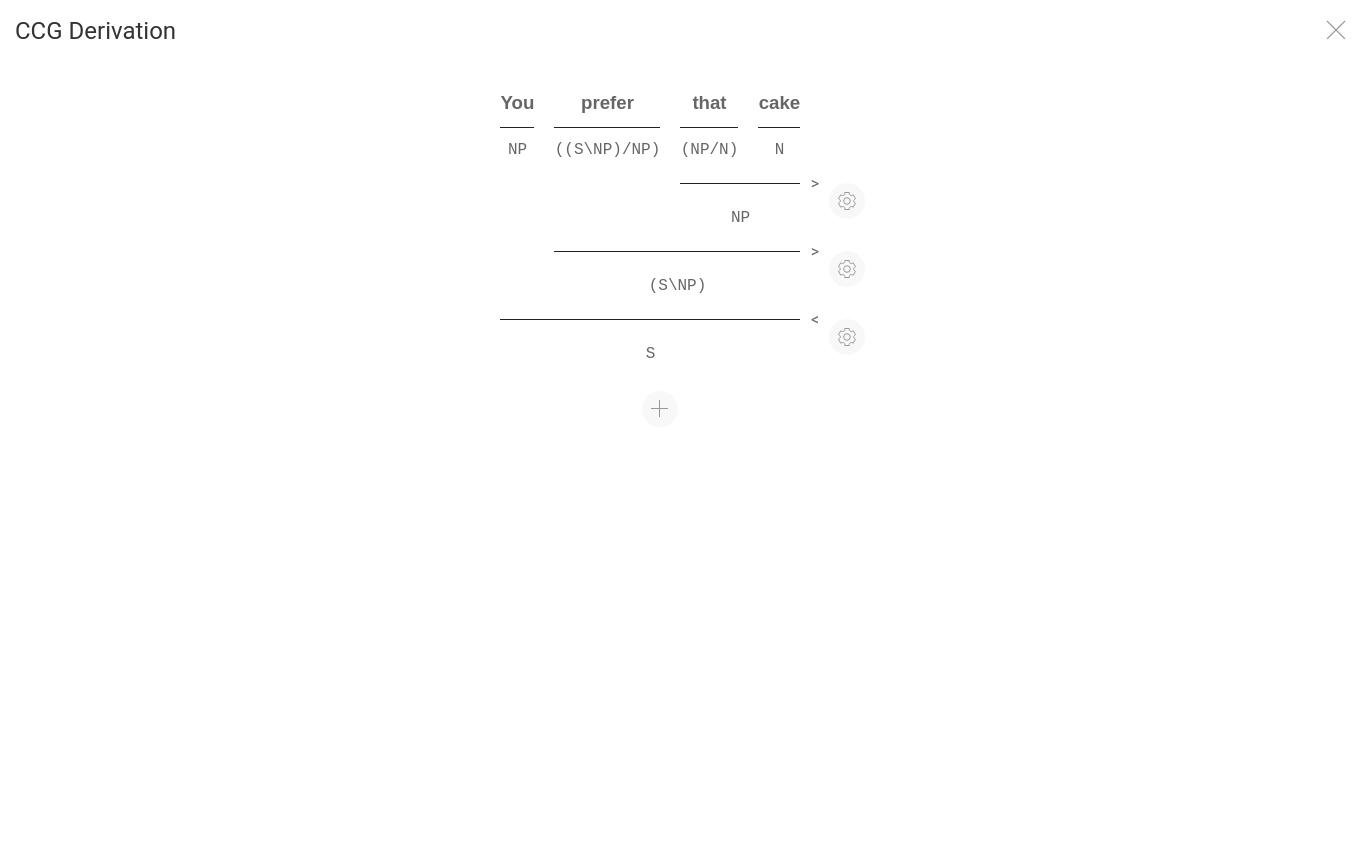
\includegraphics[width=\textwidth]{ccg-derv-generated}
  \caption{Antarmuka CCG \textit{derivation} yang telah di-\textit{generate}.}
  \label{ui:deriv-generated}
\end{figure}

\begin{figure}\centering
  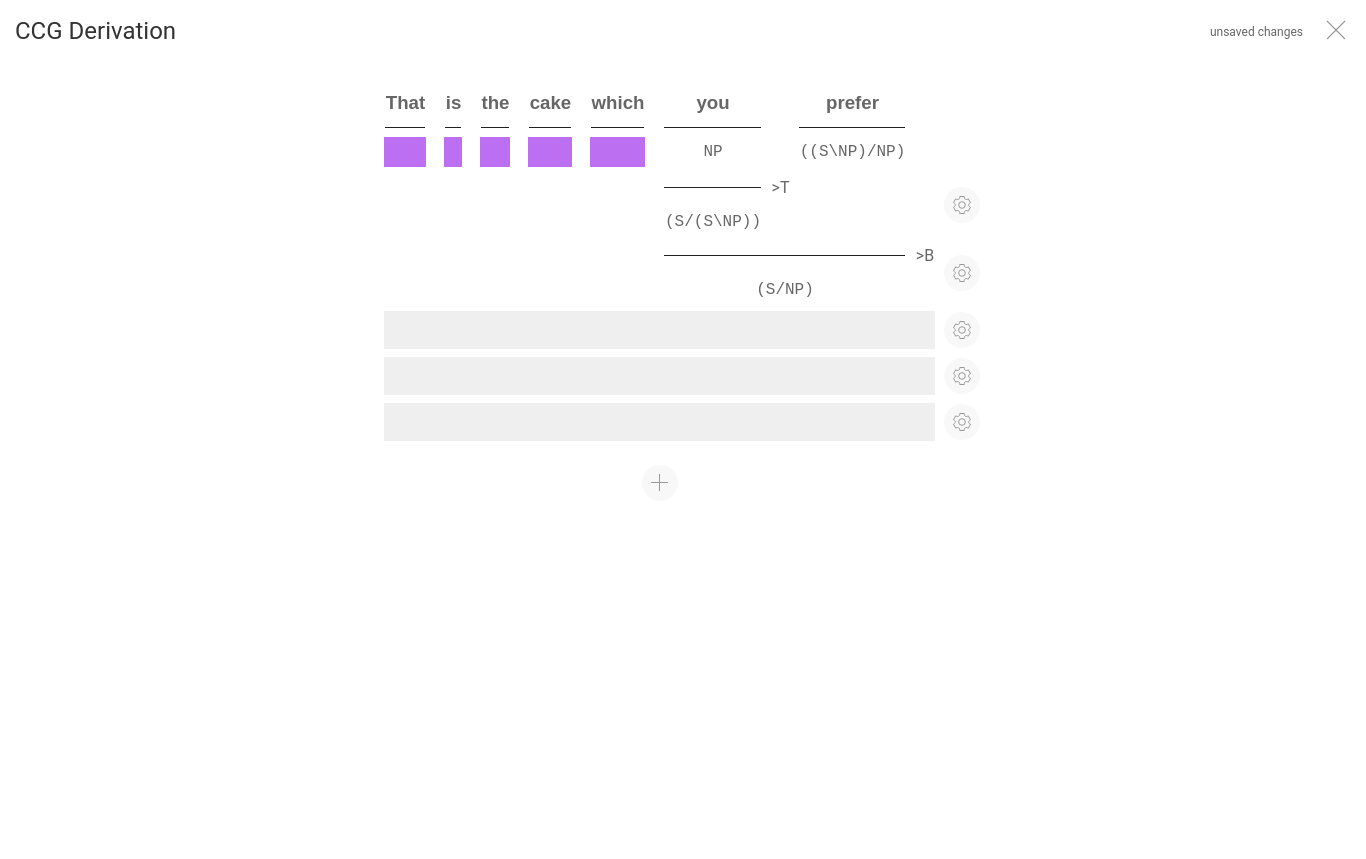
\includegraphics[width=\textwidth]{ccg-derv-progress}
  \caption{Antarmuka \textit{editable} CCG \textit{derivation} CCGtown.}
  \label{ui:deriv-progress}
\end{figure}

\begin{figure}\centering
  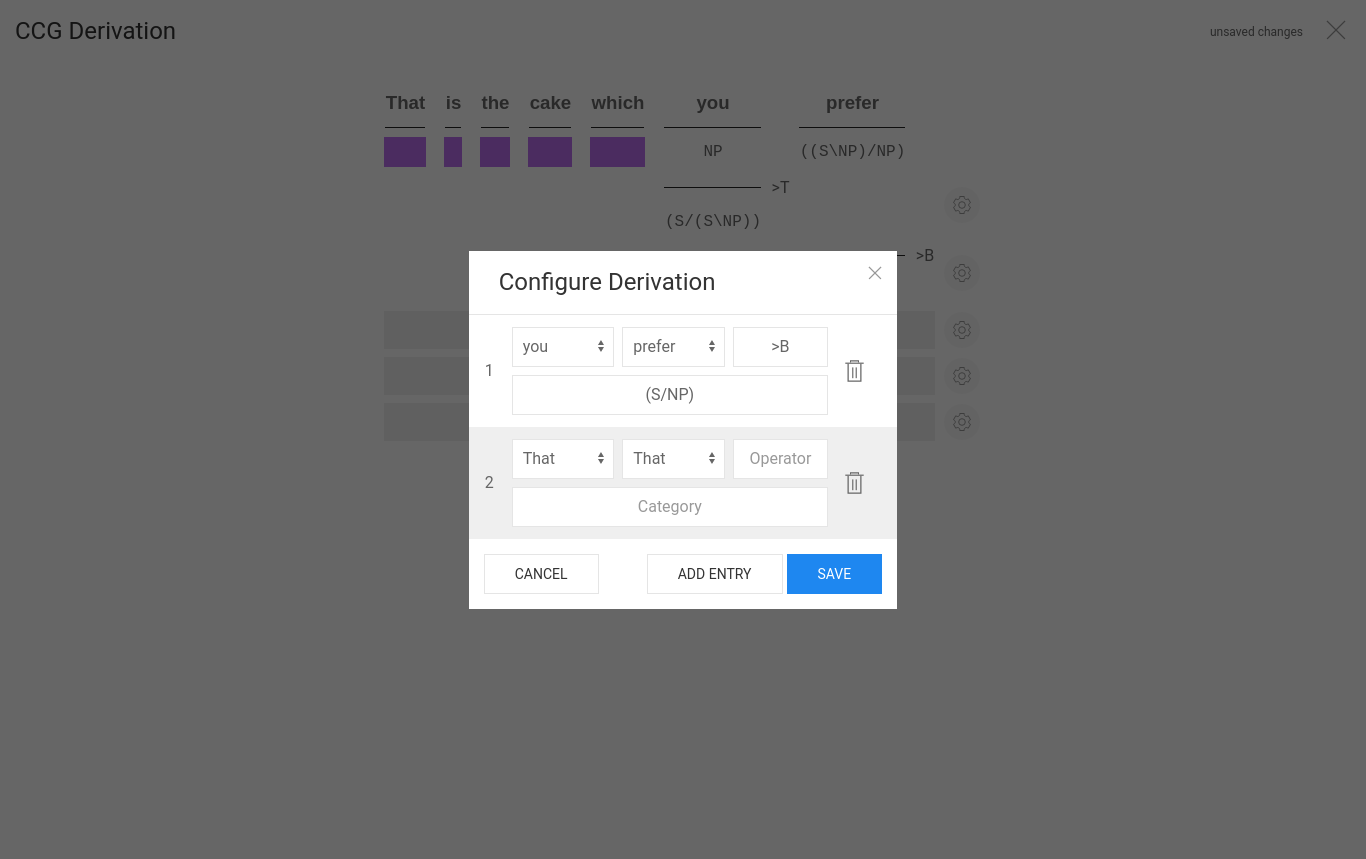
\includegraphics[width=\textwidth]{ccg-derv-configure}
  \caption{Antarmuka konfigurasi dari \textit{editable} CCG \textit{derivation} CCGtown.}
  \label{ui:deriv-configure}
\end{figure}

Selanjutnya, dengan asumsi pengguna baru saja mendaftar kemudian melakukan \textit{login},
pengguna akan dialihkan ke halaman Projects. Halaman Projects tersebut berada di dalam
\textit{empty state} karena pengguna belum membuat satupun proyek. Seperti yang dapat
dilihat pada Gambar \ref{ui:projects-empty}, pengguna dapat melihat instruksi apa yang
harus ia lakukan yang mana dalam hal ini adalah membuat proyek baru.
Sebaliknya, apabila pengguna telah membuat proyek maka tampilan yang dilihat akan
seperti pada Gambar \ref{ui:projects}. Pengguna dapat membuka halaman Editor dengan
cara melakukan klik di nama proyek maupun di ikon \textit{edit}. Selain itu,
pengguna juga dapat langsung melakukan \textit{export to JSON} melakukan klik di ikon
\textit{download}. Apabila pengguna merasa tidak lagi memerlukan suatu proyek, maka
pengguna dapat menghapusnya dengan melakukan klik di ikon \textit{trash}.

Setelah membuat proyek baru, pengguna akan melihat halaman Editor dalam
\textit{empty state} seperti yang dapat dilihat pada Gambar \ref{ui:editor-empty}.
Pada bagian kanan halaman Editor, terdapat beberapa \textit{section} yaitu
Project Detail yang dapat digunakan untuk mengubah nama proyek dan status proyek,
Automation Rules yang akan digunakan oleh NLTK untuk melakukan \textit{generate}
CCG \textit{derivation}, serta CCG Lexicons yang menampilkan statistik dari jenis
sintaksis CCG yang telah dianotasikan dan berapa kali ia dianotasikan.
Untuk dapat menambahkan kalimat baru, pengguna hanya perlu melakukan klik di
tombol "Add Sentences". Setelah itu, pengguna dapat langsung melakukan penganotasian
seperti yang terlihat pada Gambar \ref{ui:editor-annotating}. Apabila pengguna telah
memberikan anotasi ke semua token kata yang ada di kalimat tersebut, pengguna dapat
melakukan \textit{generate} CCG \textit{derivation}. Hasil dari \textit{generate} CCG
\textit{derivation} tersebut dapat dilihat pada Gambar \ref{ui:deriv-generated}.

Pengguna juga dapat langsung mengubah CCG \textit{derivation} suatu kalimat secara
langsung. Contohnya dapat dilihat pada Gambar \ref{ui:deriv-progress}.
Pengguna dapat memberikan anotasi ke token kata di \textit{modal} (\textit{editable}
CCG \textit{derivation}) tersebut. Pengguna dapat menambahkan beberapa baris kosong
sekaligus yang kemudian akan diisi oleh CCG \textit{derivation} dari kalimat tersebut.
Warna abu-abu menunjukkan bahwa konfigurasi dari CCG \textit{derivation} di baris tersebut
masih kosong. Kemudian, warna ungu menunjukkan bahwa pada bagian tersebut (baik anotasi
maupun operator) tidak diisi. Perbedaan ini diberikan untuk memberikan pengguna
\textit{awareness} mengenai mana saja bagian yang harus diisi atau dilengkapi.
Adapun konfigurasi \textit{derivation}-nya terlihat pada Gambar \ref{ui:deriv-configure}.
Dengan kemampuan ini pengguna dapat melakukan \textit{generate} kemudian apabila ada
\textit{derivation} yang dirasa kurang cocok maka pengguna dapat langsung melakukan
perubahan dengan mudah dan interaktif.

